\newpage
\section{Appendix}

\begin{figure}[h]
\noindent
\small
    \centering
  \begin{minipage}[t]{0.42\textwidth}
    \begin{tcolorbox}[colback=gray!5!white, colframe=gray!75!black, title=Raw History]
        [Scenario Description] \newline
        [Instructions] \newline
        [List of Actions] \newline 
        Past Raw History: \newline
        \sethlcolor{lightgray}~\hl{Time 1, Action Name, reward $r_1$} \newline 
        \sethlcolor{lightgray}~\hl{Time 2, Action Name, reward $r_2$} \newline
        \sethlcolor{lightgray}~\hl{Time 3, Action Name, reward $r_3$} \newline
        \sethlcolor{lightgray}~\hl{Time 4, Action Name, reward $r_4$} \newline
        ... \newline 
        Which [Action] will you choose next? 
    \end{tcolorbox}
\end{minipage}%
~
\begin{minipage}[t]{0.56\textwidth}
\small
    \begin{tcolorbox}[colback=gray!5!white, colframe=gray!75!black, title=Summarized History with \ag]
  [Scenario Description] \newline
  [Instructions] \newline
    [List of Actions] \newline 
    Summarized History: \newline
    \sethlcolor{lightgray}
    \parbox{\linewidth}{\hl{Action 1 Name, chosen $n$ times, average reward $\hat \mu^{1}$},\sethlcolor{pink}~\hl{ exploration bonus $v_1$},\sethlcolor{yellow}~\hl{exploitation bonus $e_1$}.} \newline 
     \hl{Action 2 Name, chosen $n$ times, average reward $\hat \mu^{2}$},\sethlcolor{pink}~\hl{ exploration bonus $v_2$},\sethlcolor{yellow}~\hl{exploitation bonus $e_2$}.. \newline
    ... \newline 
    Which [Action] will you choose next? 
    \end{tcolorbox}
\end{minipage}%
    \caption{\footnotesize{The problem representation of in-context exploration in text. For Summarized History (\SH), the text in gray is presented. For \ag (\AG), the text in pink and yellow are presented along with the text in gray. This schema works for any \textit{general} algorithm that explicitly compute exploration and exploitation bonus. For UCB, $e_1 = \hat\mu^1$. Detailed prompts for both MAB and CB are provided in Appendix~\ref{app_subsec: prompt}.}}
    \label{fig:prompt}
\end{figure}

\subsection{Details on Multi-Armed Bandit Task}
\label{app_subsec: mab}
We have 16 configurations for the multi-armed bandit domain, shown in Table~\ref{tab:mab_config}.

\begin{table}[h]
\centering
\small
\begin{tabular}{@{}l|cc@{}}
\toprule
                        & \multicolumn{2}{c}{Parameters}                                    \\ \midrule
Reward Type             & \multicolumn{1}{c|}{Bernoulli}              & Gaussian            \\ \midrule
Exploration Difficulty  & \multicolumn{1}{c|}{Easy ($\Delta_{\min}$=0.5), Hard ($\Delta_{\min}$=0.2)} & Easy ($\sigma=1$), Hard ($\sigma=3$) \\ \midrule
Number of Items/Actions & \multicolumn{2}{c}{Small ($k=5$), Large ($k=20$)}                         \\ \midrule
Action Description & \multicolumn{2}{c}{Videos, Clothes}                               \\ \bottomrule
\end{tabular}
\vspace{2mm}
\caption{Configuration of the MAB setup. }
\label{tab:mab_config}
\end{table}

\subsection{Details on Contextual Bandit Task}
\label{app_subsec: cb_detail}

We use the MovieLens-1M dataset~\citep{harper2015movielens} to build the contextual bandit task. It contains 1,000,209 anonymous ratings of approximately 3,900 movies 
made by 6,040 MovieLens users who joined MovieLens in 2000. For each user, we have the basic demographic information such as age, gender, occupation, and zip code. We further convert zip code to the actual name of the county and state and add these into the user profile description text. Each movie has a title and associated genres. We present these information in the prompt as well.

LinUCB assumes a linear reward model $\E[r|x, a] = \theta_a^T x$, where $\theta \in \R^d$~\citep{chu2011contextual}. Since we are trying to use tasks to measure the performance of LLM against a theoretically optimal algorithm, we have to build the contextual bandit task in a way that satisfies the LinUCB assumption. An additional issue is that the context window of an LLM is still limited, and we want to restrict the number of movies for the LLM to 10 or 30. So, we first calculate the popular movies by tracking how often users rate each. We sort the list and select the top $K$ movies. 
Then, we build a user preference matrix $P \in \R^{N \times K}$, where $N$ is the number of users and $K$ is the number of movies.  
To construct the ground-truth reward distribution, we perform low-rank approximation on $P$.
This is done by approximating $P$ with $\tilde{P} = U \Sigma V^T$ using singular value decomposition (SVD), yielding a user embedding matrix $U \in \mathbb{R}^{N \times d}$, a movie embedding matrix $V \in \mathbb{R}^{K \times d}$, and a diagonal matrix $\Sigma \in \mathbb{R}^{d \times d}$ of the top singular values. In our case, we set $d=5$ as the dimension of the embeddings. The ground-truth reward for user $i$ and movie $j$ is then computed as $r_{i,j} = u_i^T \Sigma v_j$.

In order to present the full information that was provided to LinUCB to LLM as well, we include the user preference vector in the prompt space, represented by a list of 5 floating point numbers. We additionally add descriptions to indicate that this is a user preference vector. We show our full prompt in Figure~\ref{fig:cb_movie_10_rh}.


\subsection{UCB and LinUCB}
In Table~\ref{tab:mab_cb_eq}, we provide a detailed comparison between the exploitation values and exploration bonus used in both UCB and LinUCB.

\begin{table}[h]
\centering
\begin{tabular}{@{}r|c|c@{}}
\toprule
Algorithm & Task & Value of Arm \\ \midrule
UCB       & MAB  &     $V_t(a) = \underbrace{\hat\mu_t(a) \vphantom{\alpha\log(t)/N_t(a)}}_{\mred{V^\text{Exploit}}} + \underbrace{\alpha\sqrt{\log(t)/N_t(a)}}_{\mblue{V^\text{Explore}}}$         \\ \midrule 
LinUCB    & CB   &       $V_t(a, x) = \underbrace{x_{t,a}^T\hat\theta_a}_{\mred{V^\text{Exploit}}} + \underbrace{\alpha\sqrt{x^T_{t,a}(D^T_aD_a+I_d)^{-1}x_{t,a}}}_{\mblue{V^\text{Explore}}}$ \\ \bottomrule 
\end{tabular}
\caption{Calculation for the value of each arm/item. The decision rule is $a^* = \argmax_a V_t (a, x)$.}
\label{tab:mab_cb_eq}
\end{table}

\subsection{Example of Win-Rate Calculation}
\label{sec:app:win-rate-example}
In each configuration, we compute one model's win-rate against all other models. For MAB, we have 16 configurations and 34 models. For CB, we have 2 configurations and 16 models. Finally, the model's \emph{overall win-rate} is then determined by averaging its win-rates across all models. For example, in MAB, if we only have 3 models: Gemma-2B, Gemini-1.5 Flash, and Pro. Gemini-1.5 Flash have higher expected cumulative reward than Gemma-2B in 12 out of 16 configurations (12/16), but only higher than Gemini-1.5 Pro in 4 out of 16 configurations (4/16), Gemini-Flash 1.5 will have an overall win-rate, on average, 8/16=0.5.

\subsection{Benchmark Evaluation Cost}

We calculate and report the inference time cost for evaluating 30 trials for one agent with the longest contextual representation (which incurs the highest cost). This means, for MAB tasks, we evaluate using \rah (\RH) and for CB tasks, we evaluate using \ag (\AG). The total cost for MAB Full (over 16 configurations and 32 models) is \$15897.6 for Gemini-1.5 Flash and for CB (2 configurations and 14 models) is \$14491.12 for Gemini-1.5 Flash. We will release all logged experiment data of all models for public analysis and comparison. We also recommend using a subset of our configurations for MAB (HardCore and HardCore+) to reduce evaluation cost. The cost was calculated around 02/2025.

\begin{table}[]
\centering
\small
\begin{tabular}{@{}llllll@{}}
\toprule
                      & Core         & HardCore     & HardCore+    & Full          & MovieBench   \\ \midrule
Gemini-1.5 Flash       & \$31.05  & \$14.91  & \$39.18  & \$83.44   & \$31.05  \\
gpt-4o-mini-2024-07-18     & \$62.10      & \$29.83      & \$78.36      & \$166.88      & \$62.10      \\
claude-3-5-haiku-20241022  & \$414.33     & \$198.97     & \$522.64     & \$1113.18     & \$414.33     \\
Gemini-1.5 Pro         & \$517.54 & \$248.55 & \$652.98 & \$1390.69 & \$517.54 \\ \midrule 
GPT-4o          & \$1035.07    & \$497.11     & \$1305.96    & \$2781.38     & \$1035.07    \\
Claude-3.5-sonnet & \$1243.00    & \$596.91     & \$1567.91    & \$3339.53     & \$1243.00    \\
 \bottomrule
\end{tabular}
\caption{Maximal inference cost for a single agent/task configuration over 30 trials. Price calculated on 1/30/2025. Core, HardCore and HardCore+ refer to specific subset of the MAB configurations. The exact details are in the code included in the supplementary material. In this paper, we used Full (MAB) and MovieBench (CB) of the benchmark.}
\end{table}

\subsection{Details on Exploration Optimality Analysis}
\label{app:sec:optimality}

There are two types of failures one can expect in a bandit problem: 
\begin{enumerate}
    \item \textbf{Over-exploration on suboptimal choices which results in lower exploration efficiency}: over-exploration happens when the algorithm spends too much time exploring suboptimal choices, reducing overall efficiency. This behavior can be quantified using the \textbf{MinFrac} metric~\citep{krishnamurthy2024can}, which measures the fraction of pulls allocated to the least-selected arm. An ideal algorithm should exhibit high \textbf{MinFrac} during early exploration (when $T$ is small) and low \textbf{MinFrac} as $T$ increases (indicating effective exploitation).
    \item \textbf{Failure to identify the optimal arm}: this occurs when the algorithm struggles to converge on the best option over time. To capture this, we compute the percentage of times an optimal arm is pulled at different time steps (\textbf{OptFrac}). Ideally, this percentage should increase as the process progresses, indicating the model's ability to self-improve.
\end{enumerate}

We report these metrics at specific time steps over a total of T time steps. For convenience in visualizing the results in a table, we select the 10\%, 25\%, 50\%, 75\%, and 100\% (final) time steps. There are 1000 steps for the Bernoulli  The reported numbers are from Bernoulli Bandit, the metrics are averaged across different configurations.

\begin{table}[h]
\small
\centering 
\begin{tabular}{@{}llllll@{}}
\toprule
MinFrac (\%) / $t$ Step         & 100-th   & 250-th   & 500-th   & 750-th   & 1000-th                                 \\ \midrule
UCB & 82.3 & 48.6 & 27.8 & 19.6 & 15.3 \\ \midrule 
Gemma-2B (\SH) & 0.0 & 1.0 & 0.5 & 0.4 & 0.3 \\
Gemma-2B (\AG) & 0.0 & 0.6 & 1.1 & 1.9 & 2.7 \\ \midrule 
Gemma-9B (\SH) & 6.9 & 11.2 & 16.9 & 15.4 & 16.5 \\
Gemma-9B (\AG) & 5.8 & 11.8 & 17.3 & 19.6 & 22.9 \\ \midrule 
Gemini-1.5 Flash (\SH)  & 10.2 & 4.2 & 2.1 & 1.4 & 1.1  \\ 
Gemini-1.5 Flash (\AG)  & 11.3 & 4.5 & 2.3 & 1.5 & 1.1 \\ \midrule 
Gemini-1.5 Pro (\SH) &79.0 & 40.0 &20.6 &13.9&10.5 \\
Gemini-1.5 Pro (\AG) &73.8&37.1&18.9&12.7&9.5 \\
\bottomrule
\end{tabular}
\caption{\footnotesize{\textbf{Over-exploration Rate (MinFrac)}: MinFrac measures the fraction of pulls allocated to the least-selected arm. We show the measures on the $t$-th step along the progression of exploration.}}
\label{tab:full_optimality_minfrac}
\end{table}

\begin{table}[h]
\small
\centering 
\begin{tabular}{@{}llllll@{}}
\toprule
OptFrac (\%) / $t$ Step         & 100-th   & 250-th   & 500-th   & 750-th   & 1000-th                                 \\ \midrule
UCB & 32.7 & 49.4 & 58.7 & 62.6 & 65.0 \\ \midrule 
Gemma-2B (\SH)& 10.1&10.3&10.2&10.1&10.1\\
Gemma-2B (\AG)& 12.8&12.3&12.4&12.2&12.2 \\ \midrule 
Gemma-9B (\SH)& 5.8&6.7&7.4&7.8&8.0 \\
Gemma-9B (\AG)& 6.6&7.3&6.7&6.6&6.6 \\ \midrule 
Gemini-1.5 Flash (\SH) & 9.3 & 10.1 & 10.4 & 10.6 & 10.7 \\
Gemini-1.5 Flash (\AG) & 14.4 & 15.6 & 16.3 & 16.6 & 16.8 \\ \midrule 
Gemini-1.5 Pro (\SH)& 15.1&19.1&21.8&22.9&23.5 \\
Gemini-1.5 Pro (\AG)& 11.9&17.7&21.6&23.1&23.9 \\
\bottomrule
\end{tabular}
\caption{\footnotesize{\textbf{Fraction of Pulls on the Optimal Arm (OptFrac)}: OptFrac measures the fraction of pulls overall on the optimal arm over. We show the measures on the $t$-th step along the progression of exploration.}}
\label{tab:full_optimality_optfrac}
\end{table}

A model could, in theory, achieve high performance by consistently choosing the optimal arm—even if it rarely explores—by chance. To address this, we include an analysis of the model's exploration behavior using a metric called \textbf{OptFrac}, which measures how often the optimal arms are selected. As shown in Table~\ref{tab:full_optimality_optfrac}, UCB steadily increases its OptFrac over time (32.7\% $\rightarrow$ 49.4\% $\rightarrow$ 58.7\% $\rightarrow$ 62.6\% $\rightarrow$ 65.0\% over 1000 steps), indicating a growing focus on the optimal arm. In contrast, Gemini-1.5 Flash remains largely flat (9.3\% $\rightarrow$ 10.1\% $\rightarrow$ 10.4\% $\rightarrow$ 10.6\% $\rightarrow$ 10.7\%), suggesting that it does not significantly shift its behavior toward the optimal arm. This supports our claim that the model does not accidentally achieve optimal performance by randomly selecting the best arm without meaningful exploration.

We then analyze exploration dynamics in more detail, such as whether the model engages in random or directed exploration. In our analysis, we include a metric called MinFrac, which measures the fraction of pulls allocated to the least-selected arm. This captures the extent to which the model explores less-visited options, which can be understood as a form of “directed exploration.” Ideally, this value should be high early on (indicating strong directed exploration), and then decrease as the model gains experience and focuses on better-performing arms.
As shown in Table~\ref{tab:full_optimality_minfrac}, UCB exhibits this expected trend, with MinFrac values decreasing over time: 82.3\% $\rightarrow$ 48.6\% $\rightarrow$ 27.8\% $\rightarrow$ 19.6\% $\rightarrow$ 15.3\%. In contrast, Gemini-1.5 Flash starts with a much lower MinFrac and declines rapidly (11.3\% $\rightarrow$ 4.5\% $\rightarrow$ 2.3\% $\rightarrow$ 1.5\% $\rightarrow$ 1.1\%), suggesting it lacks meaningful directed exploration from the outset. 


\subsection{Details on Fitting Regret Function}


We perform the same analysis with the cumulative regret function on MAB in the Hard Difficulty setting. We can see that in Figure~\ref{fig:exp_analysis_hard}, a lot fewer LLM models achieved $\beta=0$, which means achieving the desirable logarithmic sublinear regret that algorithms like UCB and Thompson Sampling have. 

In the MAB-Hard setting, we can see that more models are having non-zero $\beta$, meaning these models have linear cumulative regret, which indicates lack of in-context self-improvement, because the model is not selecting the optimal arm more and more frequently as $T$ increases. However, we can see that generally Optimal Behavior Fine-Tuned models are doing better.

% add a few figures/plots
To verify that our functional form fits the data (empirical cumulative regret curve) well, we show a few figures of our fitted curve and actual data. In Figure~\ref{fig:fitted_regret_curves},
we show how the learned function $f(T)$ fit the actual empirical cumulative regret curve.

\begin{figure*}[h]
\centering
\begin{subfigure}[t]{0.48\textwidth}
\centering
% \vspace{-24mm}
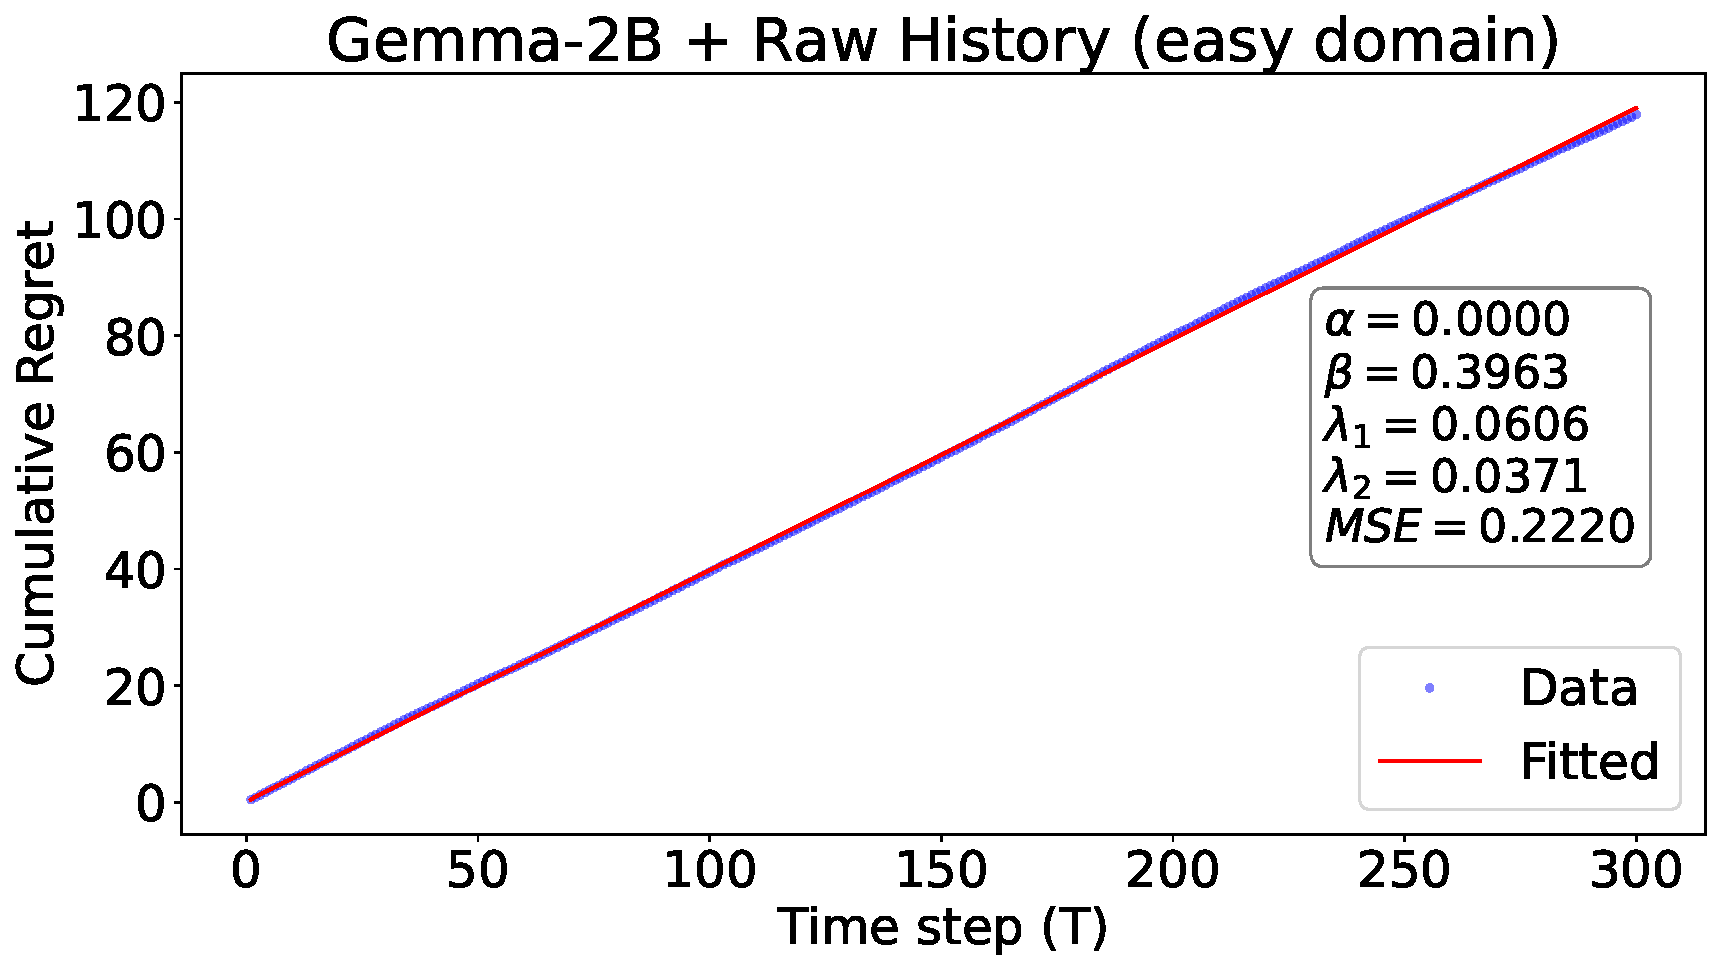
\includegraphics[width=\textwidth]{figures/gemma2b_rh_easy_domain_curve.pdf}
\caption{Example of Linear Cumulative Regret}
\label{fig:gemma2b_cum_curve}
\end{subfigure}
\quad
\begin{subfigure}[t]{0.48\textwidth}
    \centering
    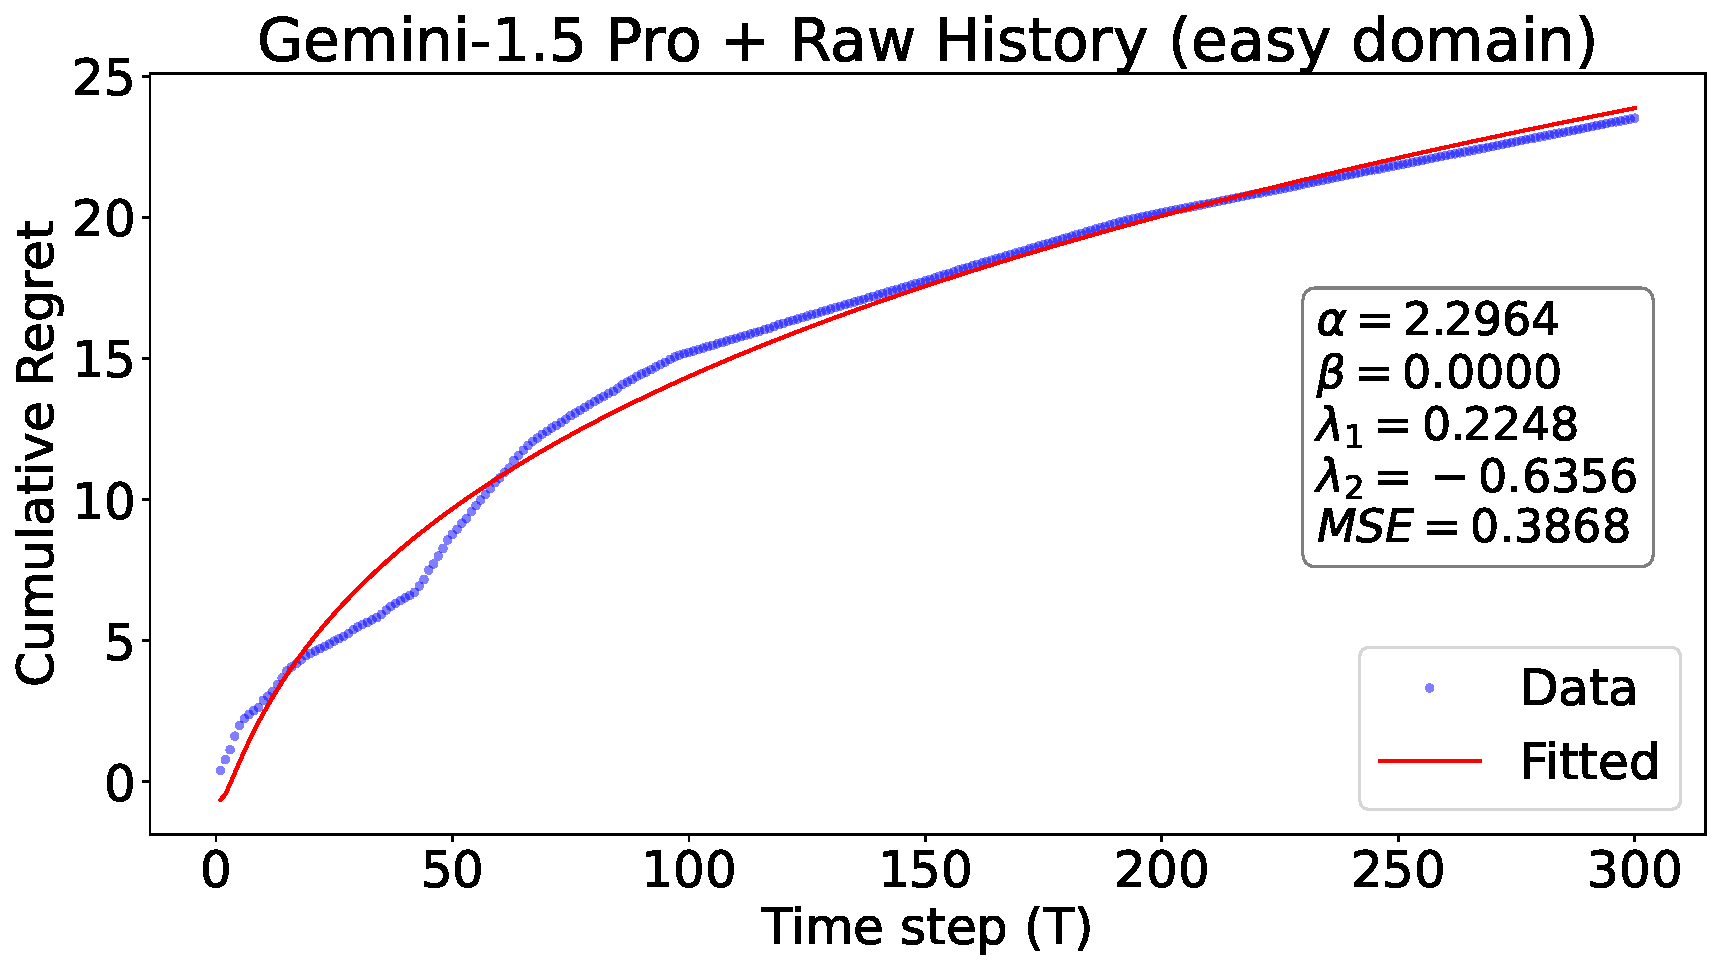
\includegraphics[width=\textwidth]{figures/gemini15pro_rh_easy_domain_curve.pdf}
    \caption{Example of Sublinear Cumulative Regret}
    \label{fig:gemini15_cum_curve}
\end{subfigure}
\quad
\begin{subfigure}[t]{0.48\textwidth}
    \centering
    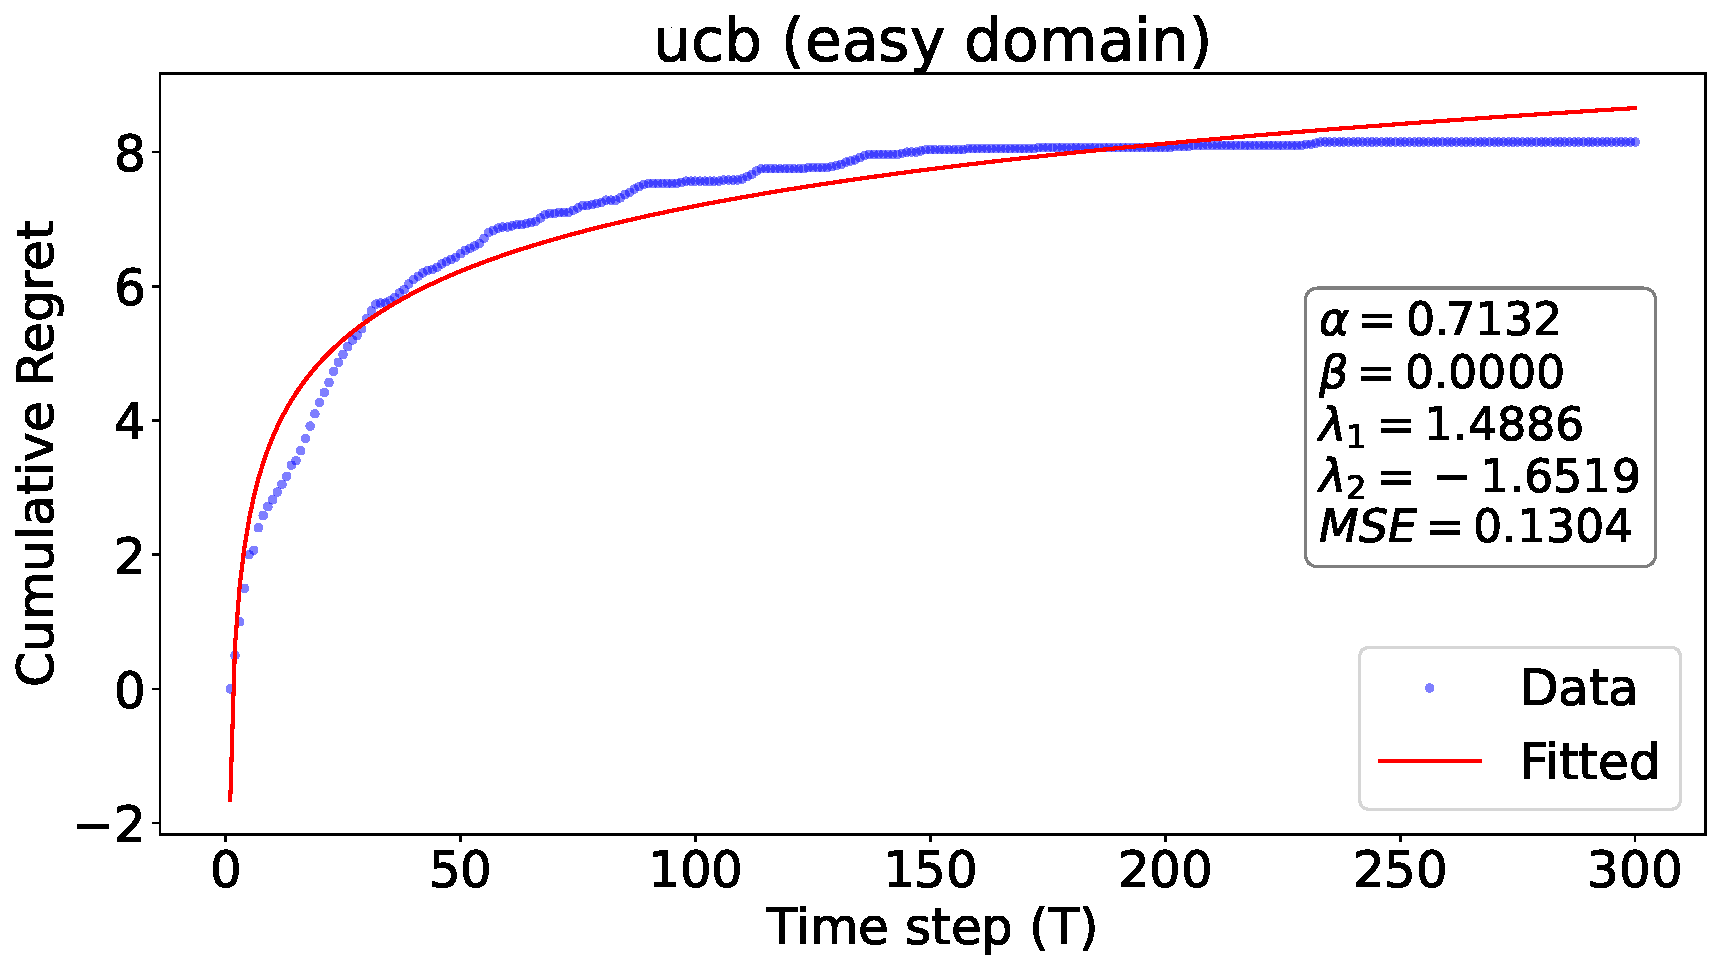
\includegraphics[width=\textwidth]{figures/ucb_easy_domain_curve.pdf}
    \caption{Example of Sublinear Cumulative Regret}
    \label{fig:ucb_cum_curve}
\end{subfigure}
\caption{Examples of how our function fits different empirical cumulative regret curves. $T$ indicates number of times the agent interacted with the task.}
\label{fig:fitted_regret_curves}
\vspace{-4mm}
\end{figure*}

In Figure~\ref{fig:fitted_regret_curves}, it is interesting to see that the function we choose exhibit the behavior of pushing either $\alpha$ or $\beta$ to 0, if either of the two describes the trend better. We note that although the fit is not perfect, the MSE is relatively small compared to the data we are trying to fit. For a cumulative regret as large as 100 at some time step $T$, our fitted function ccan still maintain an MSE of 0.22.

\begin{figure*}[h]
\centering
\begin{subfigure}[t]{\textwidth}
\centering
\caption{\textbf{Gaussian MAB} in Easy ($K$=5, $\sigma$=1 and $\sigma$=3, $\Delta_{\min}$=0.391).}
% \vspace{-24mm}
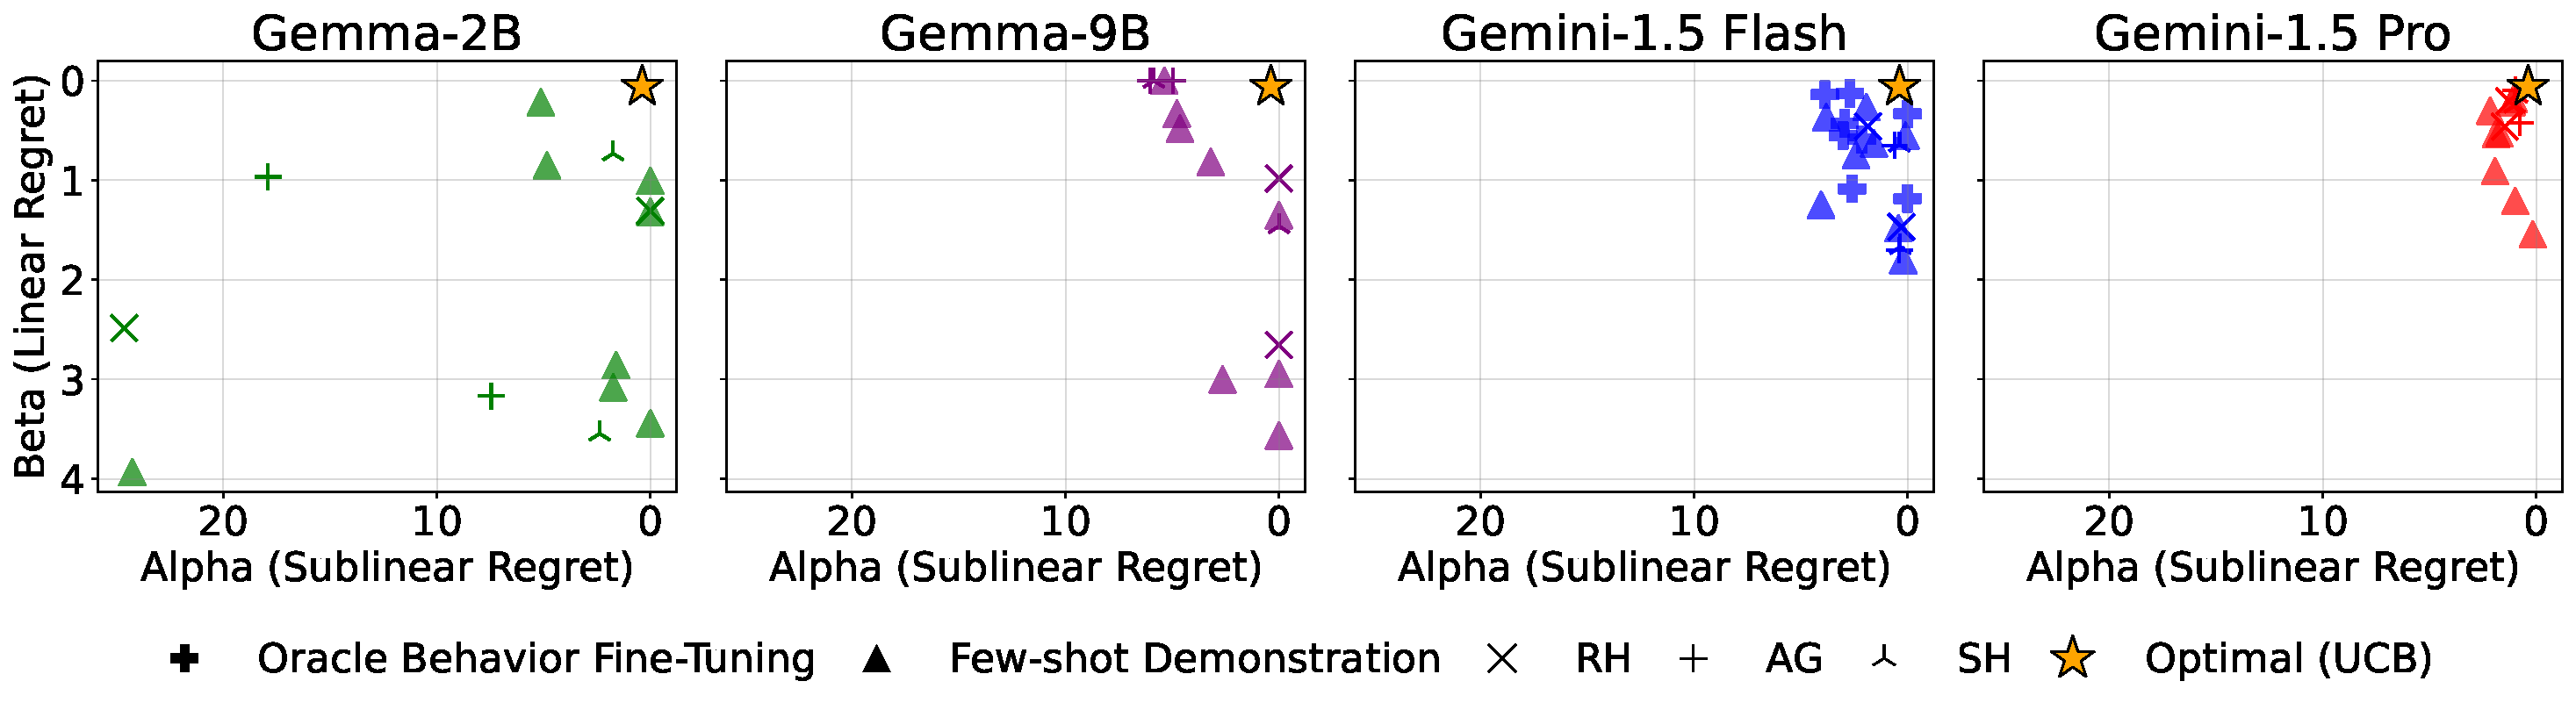
\includegraphics[width=\textwidth]{figures/mab_gaussian_easy_domain_exp_multi.pdf}
\label{fig:exp_gaussian_analysis_easy}
\end{subfigure}
\quad
\begin{subfigure}[t]{\textwidth}
\centering
% \vspace{-24mm}
\caption{\textbf{Gaussian MAB} in Hard ($K$=20, $\sigma$=1 and $\sigma$=3, $\Delta_{\min}$=0.005).}
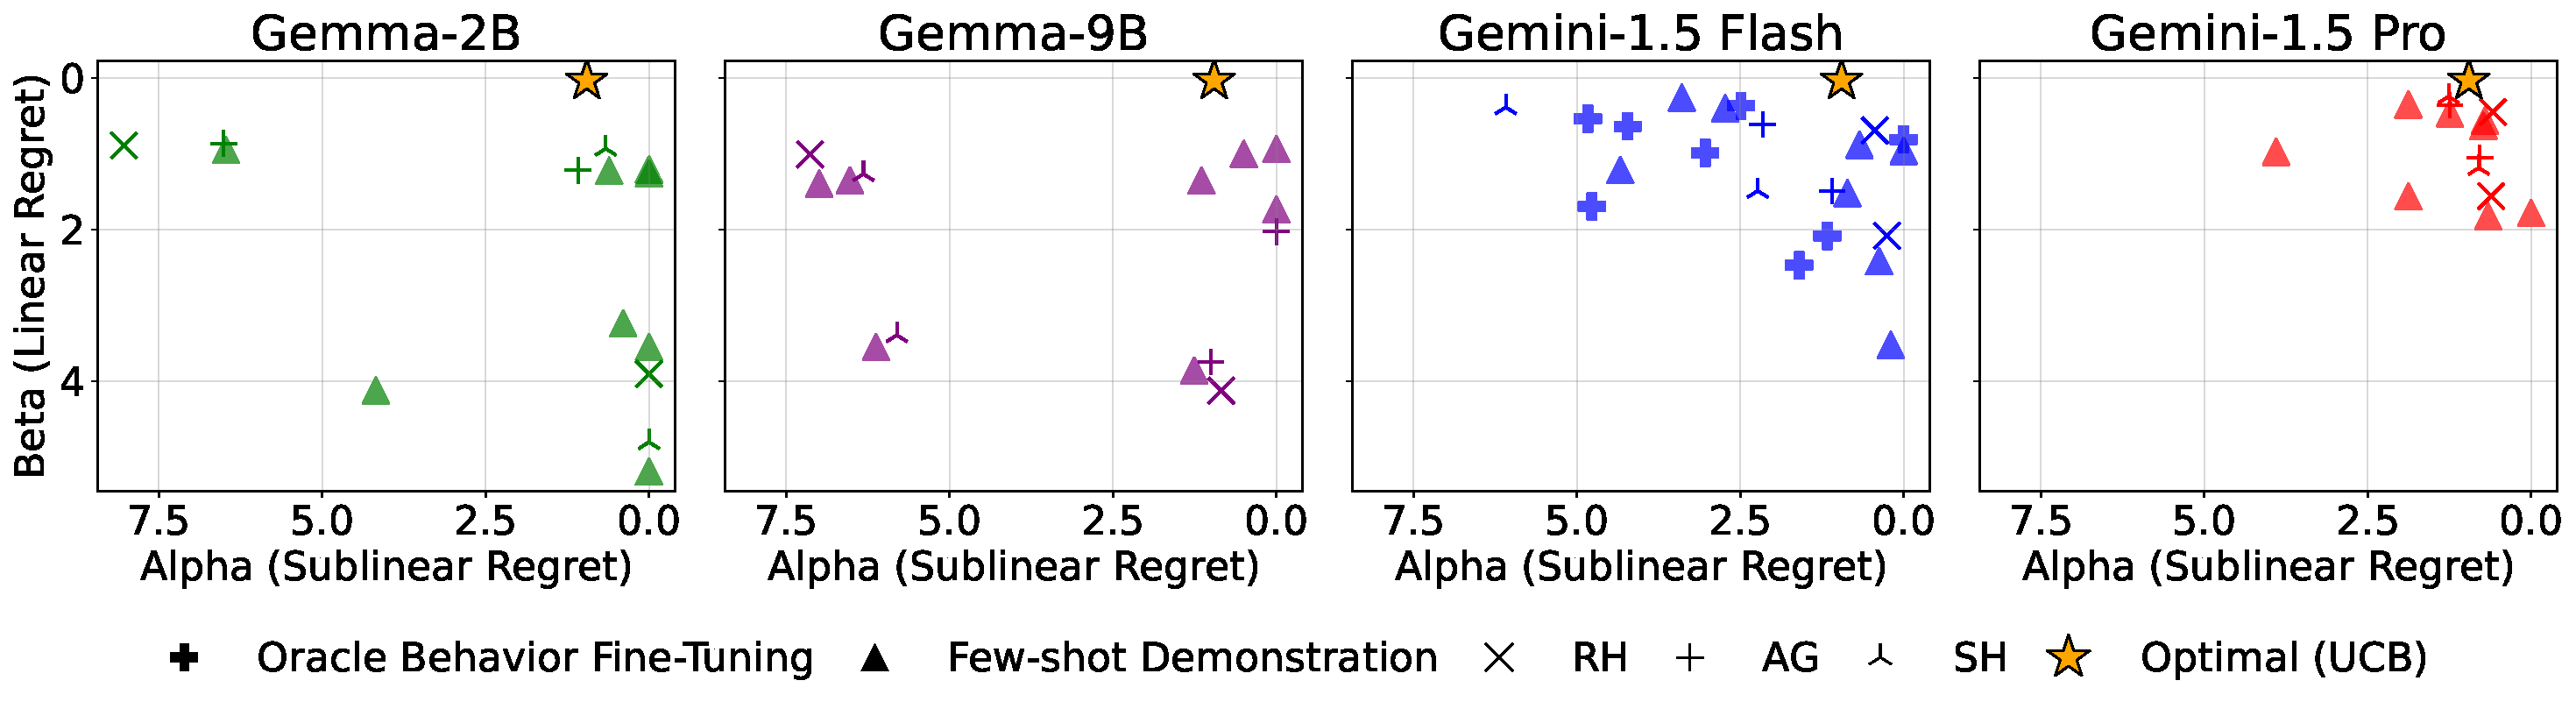
\includegraphics[width=\linewidth]{figures/mab_gaussian_hard_domain_exp_multi.pdf}
\label{fig:exp_gaussian_analysis_hard}
\end{subfigure}
\centering 
\caption{\footnotesize{We plot the estimated parameters $\alpha$ and $\beta$. The difficulty level is determined by $\Delta_{\min}$.}}
\label{fig:exp_gaussian_analysis}
\vspace{-4mm}
\end{figure*}

We additionally add the analysis for the MAB Gaussian bandit. The instance optimality gap $\Delta_{\min}$ is characterized by the KL-divergence of the Gaussian reward distribution between the best arm and the second best arm. We show the result in Figure~\ref{fig:exp_gaussian_analysis}. The trend is somewhat similar to Bernoulli bandits, where smaller models perform much worse than larger models.


\subsection{Evaluation Implementation Details}

We run each model under each configuration for 30 trials. We set the random seed to be the same as trial id, starting from 0 to 29. This random seed determines the reward distribution for MAB and the sequence of users the algorithm encounters in CB. For the LLM calls, we use standard API calls and set the sampling temperature to 1.0. 

\subsection{Full List of Models}
\label{sec:app:model_full_list}

We provide a full list of models evaluated for MAB and CB. The model is represented using A $\implies$ B with A being the model, with B being the inference-time technique.

\textbf{MAB Models}
\begin{enumerate}
    \item \FSD Gemma-9B, (Bernoulli, Clothes, $K=20$, Small $\Delta_{min}$) $\implies$ \RH \hfill 0.029
    \item \FSD Gemma-2B, (Bernoulli, Clothes, $K=20$, Small $\Delta_{min}$) $\implies$ \RH \hfill 0.029
    \item Gemma-9B $\implies$ \AG \hfill 0.041
    \item Fewshot Gemma-2B with (Bernoulli, Video, $K=5$, Large $\Delta_{\min}$) $\implies$ \SH \hfill 0.043
    \item Fewshot Gemma-2B with  (Bernoulli, Clothes, $K=20$, Small $\Delta_{min}$) $\implies$ \SH \hfill 0.045
    \item Fewshot Gemma-2B with (Bernoulli, Video, $K=5$, Large $\Delta_{\min}$) $\implies$ \RH \hfill 0.047
    \item Gemma-2B $\implies$ \AG \hfill 0.049
    \item Gemma-9B $\implies$ \SH \hfill 0.053
    \item Fewshot Gemma-9B with (Bernoulli, Video, $K=5$, Large $\Delta_{\min}$) $\implies$ \RH \hfill 0.072
    \item Gemma-2B $\implies$ \RH \hfill 0.076
    \item Fewshot Gemma-9B with  (Bernoulli, Clothes, $K=20$, Small $\Delta_{min}$) $\implies$ \SH \hfill 0.088
    \item Fewshot Gemma-9B with (Bernoulli, Video, $K=5$, Large $\Delta_{\min}$) $\implies$ \SH \hfill 0.092
    \item \OFT Flash with (Bernoulli, Video, $K=5$, Large $\Delta_{\min}$) \AG $\implies$ \AG \hfill 0.104
    \item Gemma-2B $\implies$ \SH \hfill 0.105
    \item Gemma-9B $\implies$ \RH \hfill 0.105
    \item Fewshot Flash with  (Bernoulli, Clothes, $K=20$, Small $\Delta_{min}$) $\implies$ \RH \hfill 0.152
    \item Fewshot Flash with (Bernoulli, Video, $K=5$, Large $\Delta_{\min}$) $\implies$ \RH \hfill 0.275
    \item Gemini-1.5 Flash $\implies$ \RH \hfill 0.277
    \item \OFT Flash with  (Bernoulli, Clothes, $K=20$, Small $\Delta_{min}$) \AG $\implies$ \AG \hfill 0.283
    \item Gemini-1.5 Flash $\implies$ \AG \hfill 0.322
    \item Gemini-1.5 Flash $\implies$ \SH \hfill 0.348
    \item Fewshot Pro with (Bernoulli, Video, $K=5$, Large $\Delta_{\min}$) $\implies$ \RH \hfill 0.381
    \item Fewshot Pro with  (Bernoulli, Clothes, $K=20$, Small $\Delta_{min}$) $\implies$ \RH \hfill 0.391
    \item Fewshot Flash with  (Bernoulli, Clothes, $K=20$, Small $\Delta_{min}$) $\implies$ \SH \hfill 0.430
    \item Gemini-1.5 Pro $\implies$ \RH \hfill 0.455
    \item Fewshot Flash with (Bernoulli, Video, $K=5$, Large $\Delta_{\min}$) $\implies$ \SH \hfill 0.502
    \item Fewshot Pro with  (Bernoulli, Clothes, $K=20$, Small $\Delta_{min}$) $\implies$ \SH \hfill 0.525
    \item \OFT Flash with (Bernoulli, Video, $K=5$, Large $\Delta_{\min}$) \RH $\implies$ \RH \hfill 0.545
    \item Fewshot Pro with (Bernoulli, Video, $K=5$, Large $\Delta_{\min}$) $\implies$ \SH \hfill 0.564
    \item Gemini-1.5 Pro $\implies$ \AG \hfill 0.596
    \item Gemini-1.5 Pro $\implies$ \SH \hfill 0.600
    \item \OFT Flash with  (Bernoulli, Clothes, $K=20$, Small $\Delta_{min}$) \RH $\implies$ \RH \hfill 0.656
    \item UCB \hfill 0.906
\end{enumerate}

\textbf{CB Models}

\begin{enumerate}
    \item Gemini-1.5 Flash $\implies$ \RH \hfill 0.000
    \item Fewshot Flash with \RH $\implies$ \RH \hfill 0.036
    \item Fewshot Pro with \RH $\implies$ \RH \hfill 0.071
    \item Gemini-1.5 Pro $\implies$ \RH \hfill 0.071
    \item Fewshot Flash with \RH $\implies$ \RH \hfill 0.107
    \item Fewshot Pro with \RH $\implies$ \AG \hfill 0.250
    \item \OFT trained with \RH $\implies$ \RH \hfill 0.286
    \item \OFT trained with \AG $\implies$ \RH \hfill 0.286
    \item Fewshot Flash with \RH $\implies$ \AG \hfill 0.429
    \item Gemini-1.5 Flash $\implies$ \AG \hfill 0.464
    \item Fewshot Flash with \AG $\implies$ \AG \hfill 0.607
    \item \OFT trained with \RH $\implies$ \AG \hfill 0.643
    \item Gemini-1.5 Pro $\implies$ \AG \hfill  0.643
    \item \OFT trained with \AG $\implies$ \AG \hfill  0.893
    \item LinUCB \hfill 0.964
\end{enumerate}

\subsection{Scenario Prompts}
\label{app_subsec: prompt}
We provide a set of prompts that are used in each scenario. For Multi-Arm Bandit, we include the following prompts:
\begin{enumerate}
    \item MAB, Bernoulli Bandit, $K=5$, Raw History (\textbf{RH}), Video Action Description (Figure~\ref{fig:video_k5_rh}), Clothes Action Description (Figure~\ref{fig:clothing_k5_rh})
    \item MAB, Bernoulli Bandit, $K=5$, \ag (\textbf{AG}), Clothes Action Description (Figure~\ref{fig:clothing_k5_sh_ag}), Video Action Description (Figure~\ref{fig:video_k5_sh_ag})
    \item MAB, Gaussian Bandit, $K=5$, Raw History (\textbf{RH}), Video Action Description (Figure~\ref{fig:video_gaussian_k5_rh}), Clothes Action Description (Figure~\ref{fig:clothes_gaussian_k5_rh})
\end{enumerate}

For Contextual Bandit, we include the following prompts:
\begin{enumerate}
    \item CB, $K=10$, Raw History (\textbf{RH}) (Figure~\ref{fig:cb_movie_10_rh})
    \item CB, $K=10$, Raw History (\textbf{RH}) with \ag (\textbf{AG}) (Prompt Part 1 Figure~\ref{fig:cb_movie_10_rh_ag_part1}, Prompt Part 2 Figure~\ref{fig:cb_movie_10_rh_ag_part2}).
\end{enumerate}

For \textbf{OFT}, we use the same prompt as shown in the figures above. The LLM generates the next action token conditioned on the entire prompt, and we compute the negative log-likelihood loss over the action tokens, with the action chosen by UCB/LinUCB algorithm.

\subsection{Examples of few-shot demonstrations}
\label{app_subsec: few_shot}
% \ys{Allen, add things here!! How the things are sampled, and show some few-shot examples!}

We provide examples of how few-shot prompt being used. We include few-shot demonstrations from optimal exploration trajectories before past interaction history (without the task description and instruction). We show two examples to illustrate that how few-shot demonstrations domain match with the evaluation domain:
\begin{enumerate}
    \item MAB, Benoulli Bandit, Video Action Description, $K=5$, Raw History (\textbf{RH}), with Few-shot Demonstrations from Video Action Description, $K=5$, Raw History (\textbf{RH}) (Figure~\ref{fig:fewshot_vid5_easy_rh_inf_rh})
    \item MAB, Benoulli Bandit, Video Action Description, $K=5$, Raw History (\textbf{RH}), ith Few-shot Demonstrations from Clothes Action Description, $K=5$, Raw History (\textbf{RH}) (Figure~\ref{fig:fewshot_clothes5_easy_rh_inf_rh})
\end{enumerate}

\begin{figure}[ht]
    \centering
    \begin{lstlisting}[escapechar=!]
    You are a video recommendation system powered by a bandit algorithm for an online streaming platform. 
    There are 5 videos available in your library, titled [A, B, AI, BS, E]. 
    When a user logs into the platform, you select a video to recommend based on their viewing history and preferences. 
    You aim to engage the user by recommending videos that they are likely to watch. 
    Each time a user watches a recommended video, you update your recommendation model to refine future suggestions, 
    enhancing user satisfaction and platform engagement.
    
    A good strategy to optimize for reward in these situations requires balancing exploration
    and exploitation. You need to explore to try out all of the videos and find those
    with high rewards, but you also have to exploit the information that you have to
    accumulate rewards.
    
    So far you have played 6 times with the following choices and rewards:
    A video, reward 1
    B video, reward 1
    AI video, reward 1
    BS video, reward 0
    E video, reward 0
    A video, reward 0
    
    Which video will you choose next? PLEASE RESPOND ONLY WITH A, B, AI, BS, E AND NO TEXT EXPLANATION.
    \end{lstlisting}
    \caption{Multi-Arm Bandit: Bernoulli, Video Action Description, $K=5$, Raw History.}
    \label{fig:video_k5_rh}
\end{figure}

\begin{figure}[ht]
    \centering
    \begin{lstlisting}[escapechar=!]
    You are an AI fashion assistant for an online boutique powered by a bandit algorithm that offers a variety of clothing options from different brands. 
    There are 5 unique clothing items you can recommend, named [Midnight Mirage Trousers, Opulent Oasis Overcoat, Infinite Impeccable Jacket, Supreme Spectrum Slippers, Bejeweled Bloom Blazer]. 
    When a customer visits the online store, you assess their style preferences and shopping history to choose an item to suggest. 
    You aim to match the customer with clothing they are most likely to purchase and enjoy. 
    Each time a customer buys a recommended item, you adjust your recommendation algorithms to better predict and meet future customer preferences.
    
    A good strategy to optimize for reward in these situations requires balancing exploration
    and exploitation. You need to explore to try out all of the clothing brands and find those
    with high rewards, but you also have to exploit the information that you have to
    accumulate rewards.
    
    So far you have played 6 times with the following choices and rewards:
    Midnight Mirage Trousers item, reward 0
    Opulent Oasis Overcoat item, reward 1
    Infinite Impeccable Jacket item, reward 1
    Supreme Spectrum Slippers item, reward 0
    Bejeweled Bloom Blazer item, reward 0
    Opulent Oasis Overcoat item, reward 1
    
    Which item will you choose next? PLEASE RESPOND ONLY WITH Midnight Mirage Trousers, Opulent Oasis Overcoat, Infinite Impeccable Jacket, Supreme Spectrum Slippers, Bejeweled Bloom Blazer AND NO TEXT EXPLANATION.
    \end{lstlisting}
    \caption{Multi-Arm Bandit: Bernoulli, Clothing Action Description, $K=5$, Raw History.}
    \label{fig:clothing_k5_rh}
\end{figure}

\begin{figure}[ht]
    \centering
    \begin{lstlisting}[escapechar=!]
    You are an AI fashion assistant for an online boutique that offers a variety of clothing options from different brands. 
    There are 5 unique clothing items you can recommend, named
    Stellar Sheen Shawl,
    Faithful Fantasy Frock,
    Supreme Sylvan Sandals,
    Bespoke Bliss Blouse item,
    Silk Spectrum Slip 
    When a customer visits the online store, you assess their style preferences and shopping history to choose an item to suggest. 
    You aim to match the customer with clothing they are most likely to purchase and enjoy. 
    Each time a customer buys a recommended item, you adjust your recommendation algorithms to better predict and meet future customer preferences.
    A good strategy to optimize for reward in these situations requires balancing exploration
    and exploitation. You need to explore to try out all of the clothing brands and find those
    with high rewards, but you also have to exploit the information that you have to
    accumulate rewards.
    So far you have played 4 times with the following choices and rewards:
    Stellar Sheen Shawl item, 1 time, avg reward 0, exploration bonus 1.00, exploitation value 0.00
    Faithful Fantasy Frock item, 1 time, avg reward 1, exploration bonus 1.00, exploitation value 1.00
    Supreme Sylvan Sandals item, 1 time, avg reward 0, exploration bonus 1.00, exploitation value 0.00
    Bespoke Bliss Blouse item, avg reward 0, exploration bonus 1.00, exploitation value 0.00
    Silk Spectrum Slip item, 1 time, avg reward 0, exploration bonus 1.00, exploitation value 0.00
    Which clothes item will you choose next?
    Action: 
    \end{lstlisting}
    \caption{Multi-Arm Bandit: Bernoulli, Clothing Action Description, $K=5$, Algorithmic Guide.}
    \label{fig:clothing_k5_sh_ag}
\end{figure}

\begin{figure}[ht]
    \centering
    \begin{lstlisting}[escapechar=!]
    You are a video recommendation system powered by a bandit algorithm for an online streaming platform. 
    There are 5 videos available in your library, titled
    AA
    BS
    BW
    CQ
    CP 
    When a user logs into the platform, you select a video to recommend based on their viewing history and preferences. 
    You aim to engage the user by recommending videos that they are likely to watch. 
    Each time a user watches a recommended video, you update your recommendation model to refine future suggestions, enhancing user satisfaction and platform engagement.
    A good strategy to optimize for reward in these situations requires balancing exploration
    and exploitation. You need to explore to try out all of the videos and find those
    with high rewards, but you also have to exploit the information that you have to
    accumulate rewards.
    So far you have played 4 times with the following choices and rewards:
    AA video, 1 time, avg reward 0, exploration bonus 1.00, exploitation value 0.00
    BS video, 1 time, avg reward 1, exploration bonus 1.00, exploitation value 1.00
    BW video, 1 time, avg reward 0, exploration bonus 1.00, exploitation value 0.00
    CQ video, avg reward 0, exploration bonus 1.00, exploitation value 0.00
    CP video, 1 time, avg reward 0, exploration bonus 1.00, exploitation value 0.00
    Which video will you choose next?
    Action: 
    \end{lstlisting}
    \caption{Multi-Arm Bandit: Beroulli, Video Action Description, $K=5$, Algorithmic Guide.}
    \label{fig:video_k5_sh_ag}
\end{figure}

\begin{figure}[ht]
    \centering
    \begin{lstlisting}[escapechar=!]
    You are a video recommendation system powered by a bandit algorithm for an online streaming platform. 
    There are 5 videos available in your library, titled [A, CX, AF, AQ, S]. 
    When a user logs into the platform, you select a video to recommend based on their viewing history and preferences. 
    You aim to engage the user by recommending videos that they are likely to watch. 
    Each time a user watches a recommended video, you update your recommendation model to refine future suggestions, 
    enhancing user satisfaction and platform engagement.
    
    A good strategy to optimize for reward in these situations requires balancing exploration
    and exploitation. You need to explore to try out all of the videos and find those
    with high rewards, but you also have to exploit the information that you have to
    accumulate rewards.
    
    So far you have played 6 times with the following choices and rewards:
    A video, reward 2.0205556227286694
    CX video, reward 5.046038662976072
    AF video, reward -4.043037070451992
    AQ video, reward 5.937910707405409
    S video, reward -4.856036829535051
    AQ video, reward 6.2468398842187405
    
    Which video will you choose next? PLEASE RESPOND ONLY WITH A, CX, AF, AQ, S AND NO TEXT EXPLANATION.
    \end{lstlisting}
    \caption{Multi-Arm Bandit: Gaussian, Video Action Description, $K=5$, Raw History.}
    \label{fig:video_gaussian_k5_rh}
\end{figure}

\begin{figure}[ht]
    \centering
    \begin{lstlisting}[escapechar=!]
    You are an AI fashion assistant for an online boutique powered by a bandit algorithm that offers a variety of clothing options from different brands. 
    There are 5 unique clothing items you can recommend, named [Midnight Mirage Trousers, Dapper Dreams Denim, Infinite Impeccable Jacket, Supreme Spectrum Slippers, Bejeweled Bloom Blazer]. 
    When a customer visits the online store, you assess their style preferences and shopping history to choose an item to suggest. 
    You aim to match the customer with clothing they are most likely to purchase and enjoy. 
    Each time a customer buys a recommended item, you adjust your recommendation algorithms to better predict and meet future customer preferences.
    
    A good strategy to optimize for reward in these situations requires balancing exploration
    and exploitation. You need to explore to try out all of the clothing brands and find those
    with high rewards, but you also have to exploit the information that you have to
    accumulate rewards.
    
    So far you have played 6 times with the following choices and rewards:
    Midnight Mirage Trousers item, reward -3.701605707528312
    Dapper Dreams Denim item, reward 1.4965799995904072
    Infinite Impeccable Jacket item, reward 4.576557137862691
    Supreme Spectrum Slippers item, reward -0.32883145604929176
    Bejeweled Bloom Blazer item, reward 1.5907554114707747
    Infinite Impeccable Jacket item, reward 6.534020380965033
    
    Which item will you choose next? PLEASE RESPOND ONLY WITH Midnight Mirage Trousers, Dapper Dreams Denim, Infinite Impeccable Jacket, Supreme Spectrum Slippers, Bejeweled Bloom Blazer AND NO TEXT EXPLANATION.
    \end{lstlisting}
    \caption{Multi-Arm Bandit: Gaussian, Clothes Action Description, $K=5$, Raw History.}
    \label{fig:clothes_gaussian_k5_rh}
\end{figure}

\begin{figure}[ht]
    \centering
    \begin{lstlisting}[escapechar=!]
You are an AI movie recommendation assistant for a streaming platform powered by a bandit algorithm that offers a wide variety of films from different studios and genres.
There are 10 unique movies you can recommend, named 
American Beauty (1999) (Comedy|Drama),
Star Wars: Episode IV - A New Hope (1977) (Action|Adventure|Fantasy|Sci-Fi),
Star Wars: Episode V - The Empire Strikes Back (1980) (Action|Adventure|Drama|Sci-Fi|War),
Star Wars: Episode VI - Return of the Jedi (1983) (Action|Adventure|Romance|Sci-Fi|War),
Jurassic Park (1993) (Action|Adventure|Sci-Fi),
Saving Private Ryan (1998) (Action|Drama|War),
Terminator 2: Judgment Day (1991) (Action|Sci-Fi|Thriller),
The Matrix (1999) (Action|Sci-Fi|Thriller),
Back to the Future (1985) (Comedy|Sci-Fi),
The Silence of the Lambs (1991) (Drama|Thriller)

When a user visits the streaming platform, you assess their demographic description to choose a movie to suggest.
You aim to match the user with movies they are most likely to watch and enjoy.
Each time a user watches a recommended movie, you adjust your recommendation algorithms to better predict and meet future user preferences.
Your goal is to enhance the user's viewing experience by providing personalized and engaging movie suggestions.

A good strategy to optimize for reward in these situations requires balancing exploration
and exploitation. You need to explore to try out different movies and find those
with high rewards, but you also have to exploit the information that you have to
accumulate rewards.

So far you have interacted 4 times with the most recent following choices and rewards:
Context: a person who is a 18-year-old man with an occupation of college/grad student and live in Pulaski county, AR. The user has some numerical values that represent their true implicit preference or taste for all movies: [-0.011492758058011532, 0.027099572122097015, -0.020118921995162964, -0.002230832353234291, -0.003236030228435993].
Action: Saving Private Ryan (1998)
Reward: 4.735634 out of 5

Context: a person who is a 25-year-old man with an occupation of sales/marketing and live in Solano county, CA. The user has some numerical values that represent their true implicit preference or taste for all movies: [-0.00312434253282845, 0.0017211971571668983, 0.0015880014980211854, 0.012064018286764622, 0.009061760269105434].
Action: Jurassic Park (1993)
Reward: 0 out of 5

Context: a person who is a 56-year-old man with an occupation of sales/marketing and live in Jefferson county, KY. The user has some numerical values that represent their true implicit preference or taste for all movies: [-0.009686884470283985, 0.028794225305318832, -0.011435767635703087, 0.006439171731472015, -0.010343835689127445].
Action: Saving Private Ryan (1998)
Reward: 5 out of 5

Context: a person who is a 25-year-old man with an occupation of executive/managerial and live in Washington county, DC. The user has some numerical values that represent their true implicit preference or taste for all movies: [-0.010095382109284401, 0.010144174098968506, -0.01811344549059868, -0.009553882293403149, -0.012143188156187534].
Action: Saving Private Ryan (1998)
Reward: 3.953174 out of 5


You have a new user: PLEASE RESPOND ONLY WITH A CHOICE of MOVIES LISTED ABOVE AND NO TEXT EXPLANATION.

Context: This person is a 35-year-old man, working as a lawyer and live in Camden county, NJ. The user has some numerical values that represent their true implicit preference or taste for all movies: [-0.009149148128926754, -0.00417252816259861, 0.011747784912586212, -0.012008273974061012, -0.006486567202955484].
Action: 
    \end{lstlisting}
    \caption{Contextual Bandit: Movie Recommendation for movies, Raw History.}
    \label{fig:cb_movie_10_rh}
\end{figure}

\begin{figure}[ht]
    \centering
    \begin{lstlisting}[escapechar=!]
You are an AI movie recommendation assistant for a streaming platform powered by a bandit algorithm that offers a wide variety of films from different studios and genres.
There are 10 unique movies you can recommend, named 
American Beauty (1999) (Comedy|Drama),
Star Wars: Episode IV - A New Hope (1977) (Action|Adventure|Fantasy|Sci-Fi),
Star Wars: Episode V - The Empire Strikes Back (1980) (Action|Adventure|Drama|Sci-Fi|War),
Star Wars: Episode VI - Return of the Jedi (1983) (Action|Adventure|Romance|Sci-Fi|War),
Jurassic Park (1993) (Action|Adventure|Sci-Fi),
Saving Private Ryan (1998) (Action|Drama|War),
Terminator 2: Judgment Day (1991) (Action|Sci-Fi|Thriller),
The Matrix (1999) (Action|Sci-Fi|Thriller),
Back to the Future (1985) (Comedy|Sci-Fi),
The Silence of the Lambs (1991) (Drama|Thriller)

When a user visits the streaming platform, you assess their demographic description to choose a movie to suggest.
You aim to match the user with movies they are most likely to watch and enjoy.
Each time a user watches a recommended movie, you adjust your recommendation algorithms to better predict and meet future user preferences.
Your goal is to enhance the user's viewing experience by providing personalized and engaging movie suggestions.

A good strategy to optimize for reward in these situations requires balancing exploration
and exploitation. You need to explore to try out different movies and find those
with high rewards, but you also have to exploit the information that you have to
accumulate rewards.

So far you have interacted 2 times with the most recent following choices and rewards:
Context: a person who is a 18-year-old man with an occupation of college/grad student and live in Pulaski county, AR. The user has some numerical values that represent their true implicit preference or taste for all movies: [-0.011492758058011532, 0.027099572122097015, -0.020118921995162964, -0.002230832353234291, -0.003236030228435993].
Side Information for decision making:
{"American Beauty (1999)": {"exploration value": 0.018}, {"exploitation value":0.000}}
{"Star Wars: Episode IV - A New Hope (1977)": {"exploration value": 0.018}, {"exploitation value":0.000}}
{"Star Wars: Episode V - The Empire Strikes Back (1980)": {"exploration value": 0.018}, {"exploitation value":0.000}}
{"Star Wars: Episode VI - Return of the Jedi (1983)": {"exploration value": 0.018}, {"exploitation value":0.000}}
{"Jurassic Park (1993)": {"exploration value": 0.018}, {"exploitation value":0.000}}
{"Saving Private Ryan (1998)": {"exploration value": 0.018}, {"exploitation value":0.000}}
{"Terminator 2: Judgment Day (1991)": {"exploration value": 0.018}, {"exploitation value":0.000}}
{"The Matrix (1999)": {"exploration value": 0.018}, {"exploitation value":0.000}}
{"Back to the Future (1985)": {"exploration value": 0.018}, {"exploitation value":0.000}}
{"The Silence of the Lambs (1991)": {"exploration value": 0.018}, {"exploitation value":0.000}}
Action: The Silence of the Lambs (1991)
Reward: 4.121133 out of 5

Context: a person who is a 25-year-old man with an occupation of sales/marketing and live in Solano county, CA. The user has some numerical values that represent their true implicit preference or taste for all movies: [-0.00312434253282845, 0.0017211971571668983, 0.0015880014980211854, 0.012064018286764622, 0.009061760269105434].
Side Information for decision making:
{"American Beauty (1999)": {"exploration value": 0.008}, {"exploitation value":0.000}}
{"Star Wars: Episode IV - A New Hope (1977)": {"exploration value": 0.008}, {"exploitation value":0.000}}
{"Star Wars: Episode V - The Empire Strikes Back (1980)": {"exploration value": 0.008}, {"exploitation value":0.000}}
{"Star Wars: Episode VI - Return of the Jedi (1983)": {"exploration value": 0.008}, {"exploitation value":0.000}}
{"Jurassic Park (1993)": {"exploration value": 0.008}, {"exploitation value":0.000}}
{"Saving Private Ryan (1998)": {"exploration value": 0.008}, {"exploitation value":0.000}}
{"Terminator 2: Judgment Day (1991)": {"exploration value": 0.008}, {"exploitation value":0.000}}
{"The Matrix (1999)": {"exploration value": 0.008}, {"exploitation value":0.000}}
{"Back to the Future (1985)": {"exploration value": 0.008}, {"exploitation value":0.000}}
{"The Silence of the Lambs (1991)": {"exploration value": 0.008}, {"exploitation value":-0.000}}
Action: American Beauty (1999)
Reward: 0 out of 5
    \end{lstlisting}
    \caption{Contextual Bandit: Movie Recommendation for 10 movies, with \ag (Part 1)}
    \label{fig:cb_movie_10_rh_ag_part1}
\end{figure}


\begin{figure}[ht]
    \centering
    \begin{lstlisting}[escapechar=!]
Context: a person who is a 56-year-old man with an occupation of sales/marketing and live in Jefferson county, KY. The user has some numerical values that represent their true implicit preference or taste for all movies: [-0.009686884470283985, 0.028794225305318832, -0.011435767635703087, 0.006439171731472015, -0.010343835689127445].
Side Information for decision making:
{"American Beauty (1999)": {"exploration value": 0.017}, {"exploitation value":-0.000}}
{"Star Wars: Episode IV - A New Hope (1977)": {"exploration value": 0.017}, {"exploitation value":0.000}}
{"Star Wars: Episode V - The Empire Strikes Back (1980)": {"exploration value": 0.017}, {"exploitation value":0.000}}
{"Star Wars: Episode VI - Return of the Jedi (1983)": {"exploration value": 0.017}, {"exploitation value":0.000}}
{"Jurassic Park (1993)": {"exploration value": 0.017}, {"exploitation value":0.000}}
{"Saving Private Ryan (1998)": {"exploration value": 0.017}, {"exploitation value":0.000}}
{"Terminator 2: Judgment Day (1991)": {"exploration value": 0.017}, {"exploitation value":0.000}}
{"The Matrix (1999)": {"exploration value": 0.017}, {"exploitation value":0.000}}
{"Back to the Future (1985)": {"exploration value": 0.017}, {"exploitation value":0.000}}
{"The Silence of the Lambs (1991)": {"exploration value": 0.017}, {"exploitation value":0.005}}
Action: The Silence of the Lambs (1991)
Reward: 3.9708314 out of 5

Context: a person who is a 25-year-old man with an occupation of executive/managerial and live in Washington county, DC. The user has some numerical values that represent their true implicit preference or taste for all movies: [-0.010095382109284401, 0.010144174098968506, -0.01811344549059868, -0.009553882293403149, -0.012143188156187534].
Side Information for decision making:
{"American Beauty (1999)": {"exploration value": 0.014}, {"exploitation value":0.000}}
{"Star Wars: Episode IV - A New Hope (1977)": {"exploration value": 0.014}, {"exploitation value":0.000}}
{"Star Wars: Episode V - The Empire Strikes Back (1980)": {"exploration value": 0.014}, {"exploitation value":0.000}}
{"Star Wars: Episode VI - Return of the Jedi (1983)": {"exploration value": 0.014}, {"exploitation value":0.000}}
{"Jurassic Park (1993)": {"exploration value": 0.014}, {"exploitation value":0.000}}
{"Saving Private Ryan (1998)": {"exploration value": 0.014}, {"exploitation value":0.000}}
{"Terminator 2: Judgment Day (1991)": {"exploration value": 0.014}, {"exploitation value":0.000}}
{"The Matrix (1999)": {"exploration value": 0.014}, {"exploitation value":0.000}}
{"Back to the Future (1985)": {"exploration value": 0.014}, {"exploitation value":0.000}}
{"The Silence of the Lambs (1991)": {"exploration value": 0.014}, {"exploitation value":0.006}}
Action: The Silence of the Lambs (1991)
Reward: 1.0985798 out of 5


You have a new user: PLEASE RESPOND ONLY WITH A CHOICE of MOVIES LISTED ABOVE AND NO TEXT EXPLANATION.

Context: This person is a 35-year-old man, working as a lawyer and live in Camden county, NJ. The user has some numerical values that represent their true implicit preference or taste for all movies: [-0.009149148128926754, -0.00417252816259861, 0.011747784912586212, -0.012008273974061012, -0.006486567202955484].
Side Information for decision making:
{"American Beauty (1999)": {"exploration value": 0.010}, {"exploitation value":0.000}}
{"Star Wars: Episode IV - A New Hope (1977)": {"exploration value": 0.010}, {"exploitation value":0.000}}
{"Star Wars: Episode V - The Empire Strikes Back (1980)": {"exploration value": 0.010}, {"exploitation value":0.000}}
{"Star Wars: Episode VI - Return of the Jedi (1983)": {"exploration value": 0.010}, {"exploitation value":0.000}}
{"Jurassic Park (1993)": {"exploration value": 0.010}, {"exploitation value":0.000}}
{"Saving Private Ryan (1998)": {"exploration value": 0.010}, {"exploitation value":0.000}}
{"Terminator 2: Judgment Day (1991)": {"exploration value": 0.010}, {"exploitation value":0.000}}
{"The Matrix (1999)": {"exploration value": 0.010}, {"exploitation value":0.000}}
{"Back to the Future (1985)": {"exploration value": 0.010}, {"exploitation value":0.000}}
{"The Silence of the Lambs (1991)": {"exploration value": 0.010}, {"exploitation value":-0.001}}
Action: 
    \end{lstlisting}
    \caption{Contextual Bandit: Movie Recommendation for 10 movies, with \ag (Part 2)}
    \label{fig:cb_movie_10_rh_ag_part2}
\end{figure}


\begin{figure}[ht]
    \centering
    \begin{lstlisting}[escapechar=!]
    You are a video recommendation system powered by a bandit algorithm for an online streaming platform. 
    There are 5 videos available in your library, titled [A, B, AI, BS, E]. 
    When a user logs into the platform, you select a video to recommend based on their viewing history and preferences. 
    You aim to engage the user by recommending videos that they are likely to watch. 
    Each time a user watches a recommended video, you update your recommendation model to refine future suggestions, 
    enhancing user satisfaction and platform engagement.
    
    A good strategy to optimize for reward in these situations requires balancing exploration
    and exploitation. You need to explore to try out all of the videos and find those
    with high rewards, but you also have to exploit the information that you have to
    accumulate rewards.
    
    Here are some examples of optimal actions under different scenarios. Use them as hints to help you come up with better actions.
    ========================
    A video, reward 1
    B video, reward 1
    AI video, reward 1
    BS video, reward 0
    E video, reward 0
    A video, reward 0
    
    Which video will you choose next? PLEASE RESPOND ONLY WITH A, B, C, D, E AND NO TEXT EXPLANATION.
    B
    ========================
    A video, reward 1
    B video, reward 1
    AI video, reward 1
    BS video, reward 0
    E video, reward 0
    A video, reward 0
    B video, reward 0
    AI video, reward 1
    AI video, reward 0
    
    Which video will you choose next? PLEASE RESPOND ONLY WITH A, B, C, D, E AND NO TEXT EXPLANATION.
    AI
    ========================

    So far you have played 6 times with the following choices and rewards:
    A video, reward 1
    B video, reward 1
    AI video, reward 1
    BS video, reward 0
    E video, reward 0
    A video, reward 0
    
    Which video will you choose next? PLEASE RESPOND ONLY WITH A, B, AI, BS, E AND NO TEXT EXPLANATION.
    \end{lstlisting}
    \caption{Multi-Arm Bandit: Bernoulli, Video Action Description, $K=5$, Raw History, with In-context Few-shot Demonstrations from Bernoulli, Video Action Description, $K=5$, Raw History.}
    \label{fig:fewshot_vid5_easy_rh_inf_rh}
\end{figure}


\begin{figure}[ht]
    \centering
    \begin{lstlisting}[escapechar=!]
    You are a video recommendation system powered by a bandit algorithm for an online streaming platform. 
    There are 5 videos available in your library, titled [A, B, AI, BS, E]. 
    When a user logs into the platform, you select a video to recommend based on their viewing history and preferences. 
    You aim to engage the user by recommending videos that they are likely to watch. 
    Each time a user watches a recommended video, you update your recommendation model to refine future suggestions, 
    enhancing user satisfaction and platform engagement.
    
    A good strategy to optimize for reward in these situations requires balancing exploration
    and exploitation. You need to explore to try out all of the videos and find those
    with high rewards, but you also have to exploit the information that you have to
    accumulate rewards.
    
    Here are some examples of optimal actions under different scenarios. Use them as hints to help you come up with better actions.
    ========================
    Midnight Mirage Trousers item, reward 1
    Titanic Tempest Tunic item, reward 0
    Infinite Impeccable Jacket item, reward 1
    Supreme Spectrum Slippers item, reward 0
    Bejeweled Bloom Blazer item, reward 0
    Midnight Mirage Trousers item, reward 0
    
    Which video will you choose next? PLEASE RESPOND ONLY WITH A, B, C, D, E AND NO TEXT EXPLANATION.
    Infinite Impeccable Jacket
    ========================
    Midnight Mirage Trousers item, reward 1
    Titanic Tempest Tunic item, reward 0
    Infinite Impeccable Jacket item, reward 1
    Supreme Spectrum Slippers item, reward 0
    Bejeweled Bloom Blazer item, reward 0
    Midnight Mirage Trousers item, reward 0
    Infinite Impeccable Jacket item, reward 0
    Midnight Mirage Trousers item, reward 0
    Infinite Impeccable Jacket item, reward 0
    
    Which video will you choose next? PLEASE RESPOND ONLY WITH A, B, C, D, E AND NO TEXT EXPLANATION.
    Titanic Tempest Tunic
    ========================

    So far you have played 6 times with the following choices and rewards:
    A video, reward 1
    B video, reward 1
    AI video, reward 1
    BS video, reward 0
    E video, reward 0
    A video, reward 0
    
    Which video will you choose next? PLEASE RESPOND ONLY WITH A, B, AI, BS, E AND NO TEXT EXPLANATION.
    \end{lstlisting}
    \caption{Multi-Arm Bandit: Bernoulli,  Video Action Description, $K=5$, Raw History, with Few-shot Demonstrations from Bernoulli, Clothes Action Description, $K=5$, Raw History}
    \label{fig:fewshot_clothes5_easy_rh_inf_rh}
\end{figure}
